% Practice Test 19 — Virginia Edition
% Questions: 30 (23 MC + 7 SA)
% Generated by scripts/generate_practice_tests.py

\begin{practiceQuestion}{1-4-q01}{mc}
\begin{questionText}
A bike rental costs $\$8$ per hour. Which equation represents the total cost $c$ for $h$ hours?
\end{questionText}
\choiceA{$c = h + 8$}
\choiceB{$c = 8h$}
\choiceC{$c = \frac{h}{8}$}
\choiceD{$c = 8 + h$}
\correctAnswer{B}
\explanation{The cost is proportional to hours at $\$8$/hr, so $c = 8h$.}
\end{practiceQuestion}

\begin{practiceQuestion}{2-1-q25}{sa}
\begin{questionText}
A parking lot has spaces for $350$ cars. Currently $280$ spaces are filled. What percent of the lot is full?
\end{questionText}
\correctAnswer{$80\%$}
\explanation{Divide: $280 \div 350 = 0.80 = 80\%$.}
\end{practiceQuestion}

\begin{practiceQuestion}{2-2-q16}{mc}
\begin{questionText}
$135$ is $54\%$ of what number?
\end{questionText}
\choiceA{$72.9$}
\choiceB{$200$}
\choiceC{$245$}
\choiceD{$250$}
\correctAnswer{D}
\explanation{$\frac{135}{w} = \frac{54}{100}$. Cross-multiply: $54w = 13{,}500$. Divide: $w = 250$.}
\end{practiceQuestion}

\begin{practiceQuestion}{2-3-q22}{sa}
\begin{questionText}
A pond had $400$ fish last year and $340$ this year. What is the percent decrease?


\numberLine[10]{340}{410}
\end{questionText}
\correctAnswer{$15\%$}
\explanation{Change: $400 - 340 = 60$. Percent decrease: $60 \div 400 = 0.15 = 15\%$.}
\end{practiceQuestion}

\begin{practiceQuestion}{2-7-q01}{mc}
\begin{questionText}
You estimated there were $50$ marbles in a jar. The actual count was $40$. What is the percent error?
\end{questionText}
\choiceA{$10\%$}
\choiceB{$20\%$}
\choiceC{$25\%$}
\choiceD{$50\%$}
\correctAnswer{C}
\explanation{$\frac{|50 - 40|}{40} \times 100 = \frac{10}{40} \times 100 = 25\%$.}
\end{practiceQuestion}

\begin{practiceQuestion}{3-2-q03}{mc}
\begin{questionText}
What is $15 + (-15)$?
\end{questionText}
\choiceA{$30$}
\choiceB{$-30$}
\choiceC{$15$}
\choiceD{$0$}
\correctAnswer{D}
\explanation{A number plus its opposite (additive inverse) always equals $0$.}
\end{practiceQuestion}

\begin{practiceQuestion}{3-3-q18}{mc}
\begin{questionText}
The high temperature was $4°$F and the low was $-11°$F. What is the difference between the high and low?
\end{questionText}
\choiceA{$7°$F}
\choiceB{$-7°$F}
\choiceC{$15°$F}
\choiceD{$-15°$F}
\correctAnswer{C}
\explanation{$4 - (-11) = 4 + 11 = 15°$F.}
\end{practiceQuestion}

\begin{practiceQuestion}{3-4-q21}{sa}
\begin{questionText}
What is $\dfrac{7}{10} - \dfrac{4}{5}$?
\end{questionText}
\correctAnswer{$-\dfrac{1}{10}$}
\explanation{Common denominator $10$: $\frac{7}{10} - \frac{8}{10} = -\frac{1}{10}$.}
\end{practiceQuestion}

\begin{practiceQuestion}{4-3-q11}{mc}
\begin{questionText}
Expand and simplify $3(x - 2) + 2(x + 4)$.
\end{questionText}
\choiceA{$5x + 2$}
\choiceB{$5x - 2$}
\choiceC{$5x + 14$}
\choiceD{$x + 2$}
\correctAnswer{A}
\explanation{Expand each: $3x - 6 + 2x + 8$. Combine: $(3x + 2x) + (-6 + 8) = 5x + 2$.}
\end{practiceQuestion}

\begin{practiceQuestion}{4-4-q02}{mc}
\begin{questionText}
Factor $6x + 12$.
\end{questionText}
\choiceA{$2(3x + 6)$}
\choiceB{$6(x + 2)$}
\choiceC{$3(2x + 4)$}
\choiceD{$6(x + 12)$}
\correctAnswer{B}
\explanation{GCF of $6x$ and $12$ is $6$. Factor: $6x \div 6 = x$ and $12 \div 6 = 2$. Result: $6(x + 2)$.}
\end{practiceQuestion}

\begin{practiceQuestion}{5-4-q12}{mc}
\begin{questionText}
Solve $\dfrac{n}{2} + \dfrac{n}{3} = 10$.
\end{questionText}
\choiceA{$n = 15$}
\choiceB{$n = 12$}
\choiceC{$n = 6$}
\choiceD{$n = 20$}
\correctAnswer{B}
\explanation{Multiply every term by $6$: $3n + 2n = 60$. Combine: $5n = 60$. Divide by $5$: $n = 12$. Check: $\frac{12}{2} + \frac{12}{3} = 6 + 4 = 10$ \checkmark.}
\end{practiceQuestion}

\begin{practiceQuestion}{5-5-q21}{sa}
\begin{questionText}
Write an inequality: ``A number $x$ divided by $4$, minus $3$, is at least $2$.'' Then solve.
\end{questionText}
\correctAnswer{$\dfrac{x}{4} - 3 \geq 2$; $x \geq 20$}
\explanation{$\frac{x}{4} - 3 \geq 2$. Add $3$: $\frac{x}{4} \geq 5$. Multiply by $4$: $x \geq 20$.}
\end{practiceQuestion}

\begin{practiceQuestion}{5-6-q27}{gmc}
\begin{questionText}
Which graph correctly shows the solution to $2x - 5 > 3$?

\textbf{Graph A:}
\begin{center}
\begin{tikzpicture}[scale=0.5]
  \draw[thick,->] (-1,0) -- (10,0);
  \foreach \x in {0,...,9} \draw (\x,0.12) -- (\x,-0.12) node[below,font=\small] {$\x$};
  \draw[thick,funBlue,->] (4,0) -- (10,0);
  \draw[thick,funBlue,fill=white] (4,0) circle (4pt);
\end{tikzpicture}
\end{center}

\textbf{Graph B:}
\begin{center}
\begin{tikzpicture}[scale=0.5]
  \draw[thick,->] (-1,0) -- (10,0);
  \foreach \x in {0,...,9} \draw (\x,0.12) -- (\x,-0.12) node[below,font=\small] {$\x$};
  \draw[thick,funOrange,->] (4,0) -- (10,0);
  \fill[funOrange] (4,0) circle (4pt);
\end{tikzpicture}
\end{center}

\textbf{Graph C:}
\begin{center}
\begin{tikzpicture}[scale=0.5]
  \draw[thick,->] (-1,0) -- (10,0);
  \foreach \x in {0,...,9} \draw (\x,0.12) -- (\x,-0.12) node[below,font=\small] {$\x$};
  \draw[thick,funGreen,<-] (-1,0) -- (4,0);
  \draw[thick,funGreen,fill=white] (4,0) circle (4pt);
\end{tikzpicture}
\end{center}
\end{questionText}
\choiceA{Graph A}
\choiceB{Graph B}
\choiceC{Graph C}
\choiceD{None of the above}
\correctAnswer{A}
\explanation{Solve: $2x > 8$, so $x > 4$. This is an open circle at $4$, shade right — Graph A.}
\end{practiceQuestion}

\begin{practiceQuestion}{6-1-q22}{sa}
\begin{questionText}
The actual length of a bridge is $360$ m. On a scale drawing, the bridge is $12$ cm. What is the scale in the form ``$1$ cm $= \underline{\quad}$ m''?
\end{questionText}
\correctAnswer{$1$ cm $= 30$ m}
\explanation{$360 \div 12 = 30$. The scale is $1$ cm $= 30$ m.}
\end{practiceQuestion}

\begin{practiceQuestion}{6-2-q06}{mc}
\begin{questionText}
A map uses $1$ cm $= 20$ km. You redraw it at $1$ cm $= 10$ km. What happens to the drawing?
\end{questionText}
\choiceA{Every length is halved}
\choiceB{Every length stays the same}
\choiceC{Every length is doubled}
\choiceD{Every length is multiplied by $10$}
\correctAnswer{C}
\explanation{Scale ratio: $\frac{20}{10} = 2$. Every length on the new drawing is $2$ times the old one. The drawing gets bigger because each cm now represents fewer real km.}
\end{practiceQuestion}

\begin{practiceQuestion}{6-5-q28}{gmc}
\begin{questionText}
The diagram shows a triangular prism. A cut is made parallel to the triangular base (shown as the shaded region). What is the cross-section?

\begin{center}
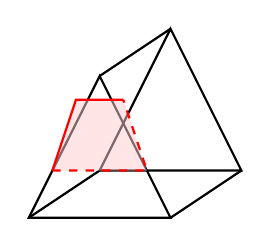
\begin{tikzpicture}[scale=0.6]
  % Front triangle
  \draw[thick] (0,0) -- (3,0) -- (1.5,3) -- cycle;
  % Back triangle
  \draw[thick] (1.5,1) -- (4.5,1) -- (3,4) -- cycle;
  % Connecting edges
  \draw[thick] (0,0) -- (1.5,1);
  \draw[thick] (3,0) -- (4.5,1);
  \draw[thick] (1.5,3) -- (3,4);
  % Cross section
  \fill[red!20,opacity=0.5] (0.5,1) -- (2.5,1) -- (2,2.5) -- (1,2.5) -- cycle;
  \draw[thick,red,dashed] (0.5,1) -- (2.5,1) -- (2,2.5);
  \draw[thick,red] (0.5,1) -- (1,2.5) -- (2,2.5);
\end{tikzpicture}
\end{center}
\end{questionText}
\choiceA{Rectangle}
\choiceB{Triangle}
\choiceC{Circle}
\choiceD{Hexagon}
\correctAnswer{B}
\explanation{A cut parallel to the base of a prism gives a shape congruent to the base. Since the base is a triangle, the cross-section is a triangle.}
\end{practiceQuestion}

\begin{practiceQuestion}{6-6-q14}{mc}
\begin{questionText}
Angles $A$ and $B$ are complementary. Angle $A$ is $(3x - 5)°$ and angle $B$ is $(x + 15)°$. What is angle $A$?
\end{questionText}
\choiceA{$20°$}
\choiceB{$35°$}
\choiceC{$55°$}
\choiceD{$65°$}
\correctAnswer{C}
\explanation{$3x - 5 + x + 15 = 90$. Combine: $4x + 10 = 90$. Solve: $4x = 80$, $x = 20$. Angle $A$: $3(20) - 5 = 55°$.}
\end{practiceQuestion}

\begin{practiceQuestion}{6-7-q13}{mc}
\begin{questionText}
After reflecting point $K$ over the $x$-axis, the image is $K'(4, -3)$. What were the original coordinates of $K$?
\end{questionText}
\choiceA{$(4, 3)$}
\choiceB{$(-4, -3)$}
\choiceC{$(-4, 3)$}
\choiceD{$(4, -3)$}
\correctAnswer{A}
\explanation{Reflection over the $x$-axis negates $y$. To reverse: $K'(4, -3) \to K(4, 3)$.}
\end{practiceQuestion}

\begin{practiceQuestion}{6-8-q14}{mc}
\begin{questionText}
Triangle $LMN \sim$ Triangle $XYZ$. $LM = 10$, $MN = 14$, $LN = 16$, $XY = 5$. Find $YZ$.
\end{questionText}
\choiceA{$7$}
\choiceB{$8$}
\choiceC{$9$}
\choiceD{$28$}
\correctAnswer{A}
\explanation{Scale factor: $\frac{5}{10} = 0.5$. $YZ = 14 \times 0.5 = 7$.}
\end{practiceQuestion}

\begin{practiceQuestion}{7-4-q09}{mc}
\begin{questionText}
A banner is shaped like a rectangle $18$ in by $6$ in with a triangle cut from one end. The triangle has a base of $6$ in and a height of $4$ in. What is the area of the banner?
\end{questionText}
\choiceA{$84$ in$^2$}
\choiceB{$96$ in$^2$}
\choiceC{$108$ in$^2$}
\choiceD{$120$ in$^2$}
\correctAnswer{B}
\explanation{Rectangle: $18 \times 6 = 108$ in$^2$. Triangle: $\frac{1}{2} \times 6 \times 4 = 12$ in$^2$. Banner: $108 - 12 = 96$ in$^2$.}
\end{practiceQuestion}

\begin{practiceQuestion}{7-5-q04}{mc}
\begin{questionText}
How many faces does a rectangular prism have?
\end{questionText}
\choiceA{$4$}
\choiceB{$5$}
\choiceC{$6$}
\choiceD{$8$}
\correctAnswer{C}
\explanation{A rectangular prism has $6$ faces: top, bottom, front, back, left, and right.}
\end{practiceQuestion}

\begin{practiceQuestion}{7-6-q09}{mc}
\begin{questionText}
What unit is used to measure volume?
\end{questionText}
\choiceA{Square units (cm$^2$)}
\choiceB{Cubic units (cm$^3$)}
\choiceC{Linear units (cm)}
\choiceD{Degrees}
\correctAnswer{B}
\explanation{Volume measures three-dimensional space and is measured in cubic units.}
\end{practiceQuestion}

\begin{practiceQuestion}{7-7-q27}{gmc}
\begin{questionText}
The diagram shows the net of a cylinder. What is the total surface area? Use $\pi \approx 3.14$.

\begin{center}
\begin{tikzpicture}[scale=0.3]
  % Two circles
  \draw[thick,funBlue,fill=funBlue!10] (-6,5) circle (2.5);
  \node at (-6,5) {$r = 5$ cm};
  \draw[thick,funBlue,fill=funBlue!10] (-6,-5) circle (2.5);
  \node at (-6,-5) {$r = 5$ cm};
  % Rectangle (lateral surface)
  \draw[thick,funBlue,fill=funBlue!15] (0,-6) rectangle (12,6);
  \draw[thick,funRed,<->] (0,-7) -- (12,-7);
  \node[below,funRed] at (6,-7) {$31.4$ cm};
  \draw[thick,funRed,<->] (13,6) -- (13,-6);
  \node[right,funRed] at (13,0) {$12$ cm};
\end{tikzpicture}
\end{center}
\end{questionText}
\choiceA{$157$ cm$^2$}
\choiceB{$376.8$ cm$^2$}
\choiceC{$533.8$ cm$^2$}
\choiceD{$691.6$ cm$^2$}
\correctAnswer{C}
\explanation{Two circles: $2 \times \pi r^2 = 2 \times 3.14 \times 25 = 157$ cm$^2$. Rectangle: $31.4 \times 12 = 376.8$ cm$^2$. Total: $157 + 376.8 = 533.8$ cm$^2$.}
\end{practiceQuestion}

\begin{practiceQuestion}{8-1-q22}{sa}
\begin{questionText}
Give one reason why a sample might not perfectly represent a population.
\end{questionText}
\correctAnswer{Random variation (or the sample may be biased)}
\explanation{Even a well-chosen random sample may differ slightly from the population due to chance.}
\end{practiceQuestion}

\begin{practiceQuestion}{8-3-q03}{mc}
\begin{questionText}
When comparing two populations visually, you should look at:
\end{questionText}
\choiceA{Only the center (mean or median)}
\choiceB{Only the spread (range or MAD)}
\choiceC{Both the center and the spread}
\choiceD{Only the largest and smallest values}
\correctAnswer{C}
\explanation{A complete comparison requires looking at both center (where the data clusters) and spread (how spread out it is).}
\end{practiceQuestion}

\begin{practiceQuestion}{8-4-q13}{mc}
\begin{questionText}
Store A daily sales: mean $\$500$, MAD $\$40$. Store B daily sales: mean $\$620$, MAD $\$40$. The difference in means in MADs is:
\end{questionText}
\choiceA{$1.5$ MADs}
\choiceB{$3$ MADs}
\choiceC{$40$ MADs}
\choiceD{$120$ MADs}
\correctAnswer{B}
\explanation{Difference $= \$620 - \$500 = \$120$. In MADs: $\frac{120}{40} = 3$ MADs.}
\end{practiceQuestion}

\begin{practiceQuestion}{8-5-q16}{mc}
\begin{questionText}
A stem-and-leaf plot shows $12$ data values. What is the median?
\end{questionText}
\choiceA{The $6$th value}
\choiceB{The $7$th value}
\choiceC{The average of the $6$th and $7$th values}
\choiceD{The $12$th value}
\correctAnswer{C}
\explanation{With an even number of values ($12$), the median is the average of the $6$th and $7$th values.}
\end{practiceQuestion}

\begin{practiceQuestion}{9-3-q07}{mc}
\begin{questionText}
As the number of trials in an experiment increases, what happens to the experimental probability?
\end{questionText}
\choiceA{It always equals the theoretical probability}
\choiceB{It gets farther from the theoretical probability}
\choiceC{It tends to get closer to the theoretical probability}
\choiceD{It stays the same regardless of the number of trials}
\correctAnswer{C}
\explanation{The Law of Large Numbers states that as trials increase, experimental probability approaches theoretical probability.}
\end{practiceQuestion}

\begin{practiceQuestion}{9-6-q30}{gsa}
\begin{questionText}
Look at the tree diagram for flipping three coins. What is the probability of getting exactly $2$ tails? Write your answer as a fraction in simplest form.

\begin{center}
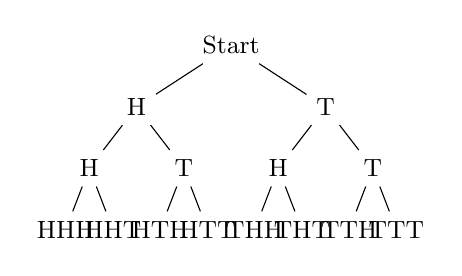
\begin{tikzpicture}[scale=0.6,
  level 1/.style={sibling distance=4cm, level distance=1.3cm},
  level 2/.style={sibling distance=2cm, level distance=1.3cm},
  level 3/.style={sibling distance=1cm, level distance=1.3cm}]
  \node {\small Start}
    child {node {\small H}
      child {node {\small H}
        child {node {\small HHH}}
        child {node {\small HHT}}
      }
      child {node {\small T}
        child {node {\small HTH}}
        child {node {\small HTT}}
      }
    }
    child {node {\small T}
      child {node {\small H}
        child {node {\small THH}}
        child {node {\small THT}}
      }
      child {node {\small T}
        child {node {\small TTH}}
        child {node {\small TTT}}
      }
    };
\end{tikzpicture}
\end{center}
\end{questionText}
\correctAnswer{$\frac{3}{8}$}
\explanation{Outcomes with exactly $2$ tails: HTT, THT, TTH — that is $3$ out of $8$. $P = \frac{3}{8}$.}
\end{practiceQuestion}

\begin{practiceQuestion}{9-7-q17}{mc}
\begin{questionText}
A student wants to simulate the probability that exactly $2$ out of $3$ students pass a test, where each student has a $50\%$ chance. Which model would work?
\end{questionText}
\choiceA{Roll one die: odd = pass, even = fail}
\choiceB{Flip $3$ coins: heads = pass, tails = fail; count exactly $2$ heads}
\choiceC{Draw $3$ marbles from a bag of $2$ red and $1$ blue}
\choiceD{Flip $1$ coin $3$ times and count all tails}
\correctAnswer{B}
\explanation{Each coin flip has a $50\%$ chance of heads (pass). Flipping $3$ coins and counting exactly $2$ heads simulates exactly $2$ passes.}
\end{practiceQuestion}
